Day two! 

\subsection{Session: Reinforcement Learning}

Mostly in the RL sessions today.

\subsubsection{A Neurally Plausible Model Learns Successor Representations in Partially Observable Environments \cite{vertes2019neurally}}

Talk by Eszter Vertes. \\

Q: How should we represent belief states? \\

A:  Distributed distributional code (DDC), and successor features (SFs)! \\

{\bf This Paper:} How to elegantly combine DDC and SFs to form distributional successor features, how to learn them, and connections to neuroscience. \\

\ddef{Successor representation}{The successor representation is given by:
\[
M^{\pi}(s_i, s_j) = \bE_\pi \left[\sum_{k=0}^\infty \gamma^k \indic\{s_{t+k} = s_j \} \mid s_t = s_i\right].
\]}

% \ddef{Distributed distributional code}{The DDC is given by:
% \[
% \mu_t(o_1, o_2, \ldots, o_t) = \bE_{q(s_t \mid o_1, \ldots, o_t)}[\psi(s_t)],
% \]
% with $\psi(s)$ a vector 
% }

% Distributional successor features:
% \[
% %DDC belief states:
% \mu = \bE[\psi(s)]
% \]
% \[
% % Distr. SFs
% M^{\pi}(\mu) = \bE_\pi
% \]

Q: How do we learn distributional successor features? \\

A: Two problems: 1) update belief states $\mu$, and 2) Learn/compute distributional SFs $M^{\pi}(\mu)$. \\

To learn the distributional SF: three methods
\begin{enumerate}
    \item Online learning: TD Learning using DDC believe states
    \item Offline learning: TD learning using simulations in latent space 
    \item Direct computation: using recurrent network dynamics.
\end{enumerate}

Contributions:
\begin{itemize}
    \item Generalize SFs to POMDPs by exploiting the relationship between DDC belief states and SFs
    \item Propose learning algorithms that span the space of model-free to model-based algorithms with biological plausibility.
    \item Highlight further connections to neuroscience data:
    \begin{itemize}
        \item Propose a novel role of hippocampal replay for learning to infer spatial location
        \item Connects threads in dopamine signals and sensory prediction errors.
    \end{itemize}
\end{itemize}

\spacerule
\subsubsection{DualDICE: Behavior-Agnostic Estimation of Discounted Stationary Distribution Corrections \cite{nachum2019dualdice}}

Talk by Ofir Nachum. \\

{\bf Central Q of the paper:} Off-policy estimation (``if I run this policy, what is the average discounted reward I will get?"). \\

$\ra$ Off-policy makes it tricky! Only get data from some other policy, may not even know which policy was followed. \\

Main Ideas:
\begin{enumerate}
    \item Reduce the off-policy estimation problem to density ratio estimation:
    \[
    d^\pi(s,a) := (1-\gamma) \sum_{t=0}
    \]
    \begin{itemize}
        \item Using importance weighting trick with a finite dataset, can compute the weighted average of the importance weights.
        \item Thus: reduces to the density ratio problem.
    \end{itemize}
    \item DualDICE operator is a zero-reward Bellman operator:
    \[
    B_\pi v(s,a) := \gamma \bE_{s' \sim T, a \sim \pi}[v(s',a)]
    \]
\end{enumerate}

The DualDICE operator then leads to a new error term that consist of minimizing squared Bellman error while also maximizing initial $\nu$-values. Desirable because objective is based on expectations from things we have access to.

\spacerule
\subsubsection{VIREL: A Variational Inference Framework for RL \cite{fellows2019virel}}

Talk by Matthew Fellows. \\

Goal; cast RL as a problem of probaltistic inference. \\

$\fa$ But: existing methods present several theoretical and practical barriers. \\

Two classical approaches:
\begin{enumerate}
    \item Pseudo-likelihood methods, which promote risk-seeking behavior
    \item Maximum entropy RL objective (Soft Actor-Critic), but optimal deterministic policies are not learned, and counterexamples show several cases when optimal RL policy can't be recovered (new result in this paper).
\end{enumerate}

Thus, new desiderata for an inference framework:
\begin{enumerate}
    \item Naturally learns optimal deterministic policies
    \item Temperature not a hyperparameter.
    \item Function approx explicitly used.
    \item Stochastic policies used for learning.
    \item Discounting easily incorporated.
    \item Optimizes the reverse form of KL divergence.
\end{enumerate}

$\implies$ Main result from the work is to outline the VIREL framework, which they show satisfies these desiderata. \\

Yields new class of Actor-Critic algorithms based on Expectation-Maximization. Evaluate on MuJoCo environments and find gains in sample efficiency.

\spacerule
\subsubsection{Unsupervised Curriculua for Visual Meta RL \cite{jabri2019unsupervised}}
% 
Talk by Kyle Hsu. \\

Objective: move RL from highly specialized learning to more general learning. \\

$\ra$ Setting is Meta-RL, in which the policy must also learn to identify the task it's in. \\

{\bf Key Component for Meta-RL;} Task distribution chosen for training in Meta-RL. \\

Q: Can we learn useful Meta-RL strategies by learning from tasks that care chosen without supervision?

A: Yes! This paper: meta-pre-training. Do unserupvised pre-training, then train. \\

Prior work: do task acquisition, then do meta-learning based on the chosen tasks. \\

This Paper; Do these two things jointly to provide an automatic curriculum. \\

Criteria for task distribution; 1) Diverse tasks, and 2) Structure in tasks. Need to trade-off between these two! Use mutual information maximization:
\[
\max_{\theta, \phi} I(\tau; z),
\]
Via an EM like approach: (E-step) updates task distribution, (M-step) do meta-training by updating policy. \\

Q: What kinds of tasks are discovered by the procedure? \\

A: Experiments in VizDoom, visualize different generated tasks. \\

\spacerule
\subsubsection{Policy Continuation with Hindsight Inverse Dynamics \cite{sun2019policy}}

Talk by Hao Sun. \\

Focus: goal-oriented reward sparse tasks. \\

$\ra$ Purely random exploration is clearly impractical due to the sparsity of the reward. But: people learn from failures, not just success! How can we leverage this idea? \\

Two ideas;
\begin{itemize}
    \item One approach: hindsight experience replay (HER) \cite{andrychowicz2017hindsight}, which explicitly tries to learn from failures.
    \item Extrapolating from success! How can we generalize from cases we were successful?
\end{itemize}

New Idea: equip inverse dynamics with hindsight (HID). But, 1-step HID is not enough, so use multi-step policy continuation to achieve multi-step optimality. \\

Experiments on simulated robot domain and grid navigation.

\spacerule
\subsubsection{Learning Reward Machines for Partially Observable RL \cite{icarte2019learning}}

Talk by Rodrigo Icarte. \\

{\bf Main Q:} How can we learn a reward machine from experience? \\

Reward Machines (RMs) are automate based reward functions, extremely useful for specifying complex behaviors. \\


This paper:
\begin{itemize}
    \item Show how to learn RMs from experience (new algorithm: LRM).
    \item Use RMs as memory for partially observable RL
    \item Extends QRMs to work under partial observability
    \item Provide theoretical and empirical analysis of LRM.
\end{itemize}

\begin{figure}[h!]
    \centering
    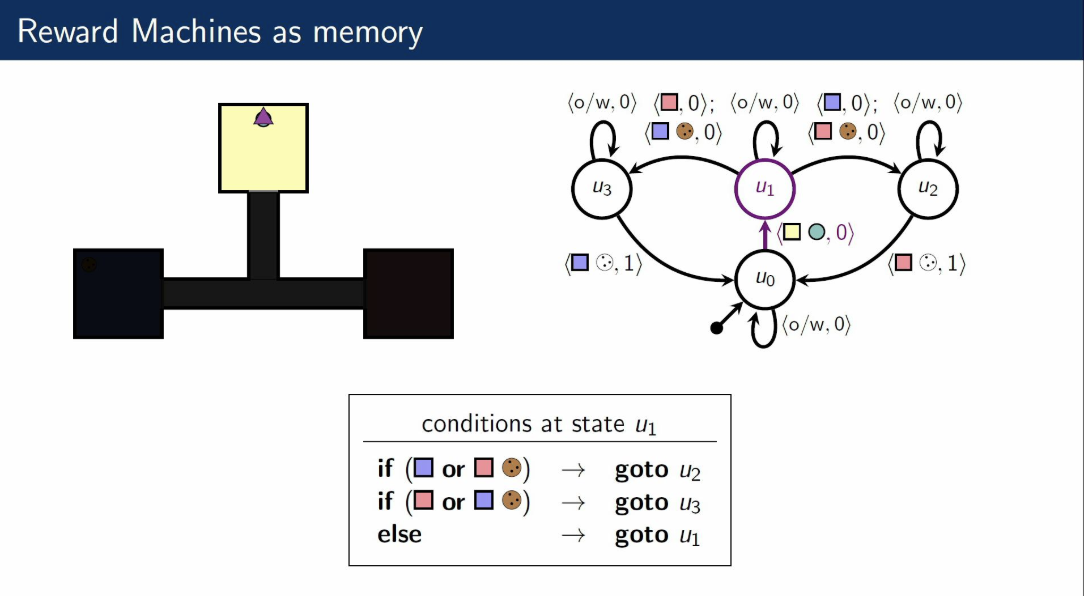
\includegraphics[width=0.7\textwidth]{figures/rm.png}
    \caption{Reward Machines as memory}
    \label{fig:rm}
\end{figure}
 
Introduce RM-DQN, a DQN variant that learns and uses a reward machine. \\

Overall approach:
\begin{itemize}
    \item Collect traces of experience
    \item Do optimization from this experience to propose a candidate RM
    \item Use the candidate RM to train an RL agent
    \item Add extra traces from new RL agent if the RM isn't perfect.
\end{itemize}

\spacerule


\subsection{Keynote: Yoshua Bengio on System 1 and System 2 in Deep Learning}

State of deep learning: amazing progress this century! \\

Q: is it enough to grow datasets, model sizes. or computer speed? \\

Q: Are wwe still far from human-level AI? \\

Some Answers: Narrow AI, sample efficiency, human-provided labels, robustness, stupid errors. Next step could be completely different from deep learning. \\

{\bf Focus Today:} There is a path from deep learning today to system 2! \\


Inspiration: ``Thinking Fast and Slow" by Daniel Kahneman.

\ddef{System 1}{Intuitive, fast unconscious non-linguistic, and habitual decision making/inference.}

Note: deep learning is good at this (system 1)!  

\ddef{System 2}{Slow, logical, sequential, conscious, linguistic, algorithmic,decision making.}

$\implies$ Claim: the future of deep learning is extending what works in system 1 to system 2. \\

Some things that are missing from deep learning right now:
\begin{enumerate}
    \item Out of distribution generalization and transfer
    \item High level cognition: need to move from system 1 to system 2.
    \begin{itemize}
        \item High level semantic representation.
        \item Compositionality.
        \item Causality.
    \end{itemize}
    \item Agent perspective:
    \begin{itemize}
        \item Machines that understand the world by building world models
        \item Knowledge-seeking
    \end{itemize}
\end{enumerate}

{\bf Theme Today:} These three areas are intimately connected, and these connections can help us identify a path forward in AI/ML research. \\

The talk:
\begin{enumerate}
    \item ML Goal: Handle Changes in Distribution
    \item System 2 Basics:  Attention and Consciousness
    \item Consciousness Prior:  Sparse Factor Graph
    \item Theoretical  framework:  meta-learning,  localized  change hypothesis→causal discovery
    \item  Compositional DL architectures
\end{enumerate}

% Consciousness Funtionalities: Roadmap for Priors Empowering System 2
\spacerule
\subsubsection{ML Goal: Handle Changes in Distribution}

Classical ML theory is {\it for i.i.d. data}. Without this assumption we can't say anything about generalization. \\

$\ra$ Naturally, this assumption is unrealistic. \\

But: {\it ``Nature does not shuffle the data, we shouldn't"}
-- Leon Bottou (ICML 2019 Keynote). \\

Out of distribution generalization and transfer breaks the i.i.d. hypothesis, so what do we do? Can we replace it with something else? \\

A: Agent learning needs out-of-distribution (OOD) generalization. \\


Why? Well: Agents face non-stationarities resulting from 1) their actions, 2) actions of other agents, 3) different places, times, sensors, and so on. \\

{\bf Claim:} compositionality helps OOD generalization. \\

$\ra$ Different forms of compositionality, each comes ith different exponential advantages. See, for instance:
\begin{itemize}
    \item Distributed representations
    \item Composition of layers in deep nets DAVEEITE: Montufar NeurIPS 2014
    \item Systematic generalization in language, analogies, abstract reasoning.
\end{itemize}

Q: So, how do we do systematic generalization? \\

A: Important to dynamically recombing existing concepts, {\it even when new combinations have 0 probability under training distributions}. Think of a science fiction scenario! We don't live that, but can still imagine it and draw meaningful insights from it. \\

$\ra$ Current methods are not effective for this. \\

Q: How does what you are proposing contrast with the symbolic AI program? \\

A: Avoids pitfalls of classical AI rule-based symbol manipulation. That is, we need the following:
\begin{itemize}
    \item Need efficient large-scale learning
    \item Need semantic grounding in system 1
    \item Need distributed representations for generalization
    \item Need efficient (trained) search for both systems
    \item Need systems that can properly handle uncertainty in the world.
\end{itemize}

But, we also want:
\begin{itemize}
    \item Systematic generalization
    \item Factorizing knowledge in small exchangeable pieces
    \item manipulating variables, instances, references, and indirection.
\end{itemize}


\spacerule
\subsubsection{System 2 Basics: Attention and Consciousness}

{\bf Claim:} Key ingredient for consciousness is {\it attention}. \\

Q: What is attention? \\

A: Focus on one or a few elements at a time. Content-based soft attention is convenient because we can backprop to learn where to attend. Lots of benefits:
\begin{enumerate}
    \item Neural Machine Translation revolution \cite{bahdanau2014neural}.
    \item SOTA in NLP, self attention/transformers
    \item Memory-extended neural nets
    \item Address vanishing gradients
    \item Operating on unordered sets.
\end{enumerate}

$\ra$ Attention creates a {\it dynamic} connection between two layers of a neural net. \\

From Attention to Consciousness:
\begin{itemize}
    \item ``C"-word is not taboo anymore in cognitive neuroscience
    \item One main theory: ``Global Workspace Theory" \cite{baars2005global}.
    \begin{itemize}
        \item Bottleneck of conscious processing
        \item Selected item is broadcast, stored in short-term memory, conditions perception and action
        \item System 2 like sequential processing, conscious reasoning and planning and imagination.
    \end{itemize}
\end{itemize}

Q: So how can we connect these ideas to machine learning? (can the two communities help each other?) \\

A: ML can help us formalize, in a mechanistic way, and test specific hypothesized functionalities of consciousness. This could: 1) get the magic out of consciousness, 2) understand evolutionary advantage of consciousness by grounding it to computation and statistics. \\

Concsciousness closely related to language: we assign consciousness from humans reporting, and moreover, high level representations are deeply connected to language. \\

$\ra$ Thus, a connection between System 1 and System 2: meaning anchored in low-level perception and action. \\

So need {\it grounded language learning}, such as BabyAI \cite{chevalier2018babyai}.

\spacerule
\subsubsection{Consciousness Prior: Sparse Factor Graph}

Q: So what kinds of priors and structures can we use to get our learning algorithms to use these kinds of abilities? \\

Proposal one: the consciousness prior \cite{bengio2017consciousness}.
\begin{itemize}
    \item Attention: to form conscious state and thought
    \item A thought is a low-dimensional object, few selected aspects of the unconscious state
    \item Need 2 high level states: 1) large unconscious state, and 2) tiny conscious state.
    \item Part of inference mechanism with respct to joint distribution of high-level variables.
\end{itemize}

Concretely, the consciousness prior proposes a {\it sparse factor graph}, where nodes are variables, and edges represent relations between these variables.\\

Why is this a reasonable hypothesis?
\begin{itemize}
    \item Property og high-level variables which we manipulate with language; we can predict {\it some} given very few others.
    
    For instance: ``if I drop the ball, it will fall on the ground"
    
    \item Disentangled factors are not marginally independent (ball, hand, etc)
    \item Prior: sparse factor graph imposes a joint distribution between high-level variables.
    
    \item Note: this prior does not work in the space of pixels.
\end{itemize}


% idea:
% \[
% P(V) \propto \Prod_k \phi_k(V_{sk})
% \]


\spacerule
\subsubsection{Theoretical framework: meta-learning, localized change hypothesis $\ra$ causal discovery}

Meta-Learning (or ``learning to learn"): having multiple time scales of learning.
\begin{itemize}
    \item Bi-level optimization:
    \begin{itemize}
        \item Inner Loop of learning that outputs a loss
        \item Outer loop: continual learning that optimizes the loss from the inner loop
    \end{itemize}
    \item Examples: evolution \& individual learning, Lifelong learning and adaptation to new environments.
\end{itemize}

Q: what causes changes in distribution? \\

{\bf Hypothesis to replace i.i.d. assumption:} the ``localized change hypothesis":

\ddef{Localized Change Hypothesis}{``changes are consequences of an intervention on a few causes or mechanisms." \cite{scholkopf2012causal}}

Then: use OOD generalization as a training signal for factorizing knowledge \cite{bengio2019meta}.
\begin{itemize}
    \item A meta-transfer objective for learning to disentangle causal mechanisms
    \item Learning whether A causes B or vice-versa
    \item Learning to disentangle (A,B) from (X,Y)
    \item Exploit changes in distribution and speed of adaptation to guess causal direction.
\end{itemize}

Newer work: Learning neural causal models from unknown interventions \cite{ke2019learning}. \\

$\ra$ Learning small causal graphs to avoid exponential explosion of number of graphs by parameterizing factorized distribution over graphs. \\

Note: attacking this problem in a very deep learning friendly way. Can plug into the deep learning tools that work already.



\spacerule
\subsubsection{Compositional DL architectures}



Recurrent Independent Mechanisms (RIMs) \cite{goyal2019recurrent}: modularize computation and operate on sets of named and typed objects.
\begin{itemize}
    \item multiple recurrent sparsely interacting modules, each with dynamics and object input-outputs
    \item Results: much better OOD generalization!
    \item Also RIMs as a replacement for LSTM in PPO, find improvements in Atari.
\end{itemize}



Summary: Hypotheses for Conscious Processing by Agents, Systematic Generalization:
\begin{itemize}
    \item Sparse factor graph in space of high-level semantic variables
    \item Semantic variables are causal: agents, intentions, controllable objects
    \item Shared rules across instance tuples
    \item Distributional changes from localized causal interventions.
    
    $\ra$ Changes are mostly localized {\it if you represent things in the right space}
    
    \item Things that are preserved across changes in distribution are the fundamental stable aspects of the world. Meaning should target these aspects.
\end{itemize}

Conclusions:
\begin{itemize}
    \item Time is ripe for ML/AI to explore consciousness
    \item Could bring new priors to help systematic and OOD generalization
    \item Could benefit cognitive neuroscience too
    \item Would allow us to expand deep learning from system 1 to system 2.
\end{itemize}

% Q\&A:
% Q: Broad consensus among moral philosophers is that conscisouness is what is necessary for something to be a moral patient. \\

% A: Today I've only talked about the easy problem of consciousness. In Neuro, lots of work on this for awhile.



